\chapter{Material complementario del experimento de benchmarks}
\label{app:benchmarks_complementario}

Este anexo recoge el material metodológico y gráfico del experimento de benchmarks que se ha retirado del cuerpo principal para mantener la memoria dentro del límite de extensión. En el Capítulo~\ref{chap:diseno_experimental} se conservan los elementos principales del análisis: el cuadro de benchmarks, la configuración general del experimento, el resumen del \emph{incumbent}, la evolución del \emph{incumbent}, el resumen predictivo y la jerarquía de factores experimentales.

\section{Dominio detallado del benchmark Borehole}
\label{app:dominio_borehole}

\begin{table}[htbp]
\centering
\small
\caption{Dominio del benchmark Borehole.}
\label{tab:app_dominio_borehole}
\renewcommand{\arraystretch}{1.15}
\begin{tabularx}{\textwidth}{@{}p{1.8cm} X p{3.4cm}@{}}
\toprule
\textbf{Variable} & \textbf{Descripción} & \textbf{Dominio} \\
\midrule
\(r_w\)
& Radio del pozo
& \([0.05, 0.15]\) \\

    \(r\) 
    & Radio de influencia 
    & \([100, 50000]\) \\

    \(T_u\) 
    & Transmisividad del acuífero superior 
    & \([63070, 115600]\) \\

    \(H_u\) 
    & Carga piezométrica superior 
    & \([990, 1110]\) \\

    \(T_l\) 
    & Transmisividad del acuífero inferior 
    & \([63.1, 116]\) \\

    \(H_l\) 
    & Carga piezométrica inferior 
    & \([700, 820]\) \\

    \(L\) 
    & Longitud del pozo 
    & \([1120, 1680]\) \\

    \(K_w\) 
    & Conductividad hidráulica del pozo 
    & \([9855, 12045]\) \\
    \bottomrule 
\end{tabularx}

\end{table}
\FloatBarrier
\newpage
\section{Flujo del proceso de \emph{infill}}
\label{app:flujo_infill}

\begin{figure}[htbp]
\centering
\resizebox{0.95\textwidth}{!}{%
\begin{tikzpicture}[
box/.style={
rectangle,
rounded corners=3pt,
draw=black,
align=center,
minimum width=4.0cm,
minimum height=1.05cm,
inner sep=4pt,
font=\small
},
arrow/.style={
-{Latex[length=2mm]},
thick
},
looparrow/.style={
-{Latex[length=2mm]},
thick,
dashed,
rounded corners=6pt
},
looplabel/.style={
font=\small,
fill=white,
inner xsep=4pt,
inner ysep=1pt
}
]

    \node[box] (init) at (0,0) {
        \textbf{Diseño inicial}\\
        \(\mathcal{D}_n=\{(\bm{x}_i,y_i)\}_{i=1}^{n}\)
    };

    \node[box] (train) at (5.4,0) {
        \textbf{Entrenar GP}\\
        sobre \(\mathcal{D}_n\)
    };

    \node[box] (pred) at (10.8,0) {
        \textbf{Predicción}\\
        \(\mu(\bm{x}),\,\sigma(\bm{x})\)
    };

    \node[box] (ei) at (10.8,-2.25) {
        \textbf{Calcular EI}\\
        minimización
    };

    \node[box] (opt) at (5.4,-2.25) {
        \textbf{Optimizar EI}\\
        \(\bm{x}_{\mathrm{next}}=\operatorname*{arg\,max}_{\bm{x}} EI(\bm{x})\)
    };

    \node[box] (eval) at (0,-2.25) {
        \textbf{Evaluar benchmark}\\
        \(y_{\mathrm{next}}=f(\bm{x}_{\mathrm{next}})\)
    };

    \node[box] (update) at (0,-4.5) {
        \textbf{Actualizar datos}\\
        \(\mathcal{D}_{n+1}=\mathcal{D}_n \cup\)\\
        \(\{(\bm{x}_{\mathrm{next}},y_{\mathrm{next}})\}\)
    };

    \node[box] (metrics) at (5.4,-4.5) {
        \textbf{Evaluar métricas}\\
        test y mejor valor observado
    };

    \draw[arrow] (init) -- (train);
    \draw[arrow] (train) -- (pred);
    \draw[arrow] (pred) -- (ei);
    \draw[arrow] (ei) -- (opt);
    \draw[arrow] (opt) -- (eval);
    \draw[arrow] (eval) -- (update);
    \draw[arrow] (update) -- (metrics);

    \coordinate (loopA) at (13.8,-4.5);
    \coordinate (loopB) at (13.8,1.85);
    \coordinate (loopC) at (5.4,1.85);

    \draw[looparrow]
        (metrics.east)
        -- (loopA)
        -- (loopB)
        -- node[looplabel, above, midway]
            {Repetir hasta agotar el presupuesto de \emph{infill}}
        (loopC)
        -- (train.north);

\end{tikzpicture}%
}
\caption[Flujo del proceso de infill]{Flujo del proceso de \emph{infill} empleado en los benchmarks sintéticos. En cada iteración se entrena una configuración GP con las observaciones disponibles, se calcula EI, se selecciona el siguiente punto maximizando dicho criterio, se evalúa la función benchmark y se actualiza el conjunto de entrenamiento.}
\label{fig:app_flujo_infill}

\end{figure}
\FloatBarrier

\subsection*{Descripción detallada del proceso de \emph{infill}}

El proceso de \emph{infill} reproduce un escenario de optimización con evaluaciones costosas, donde cada nuevo punto debe seleccionarse de forma informada. En este experimento, la función objetivo se formula como un problema de minimización, por lo que la mejora esperada se calcula respecto al mejor valor observado hasta el momento.

En cada iteración, el GP se ajusta con el conjunto de observaciones disponible \(\mathcal{D}_n\) y se calcula el criterio EI sobre el dominio de búsqueda. Aunque la función objetivo se minimiza, EI se maximiza, ya que se busca el punto con mayor mejora esperada:

\[
\bm{x}_{\mathrm{next}}
=
\operatorname*{arg\,max}_{\bm{x}\in\mathcal{X}} (EI(\bm{x})).
\]

La maximización de EI se realiza mediante \emph{Differential Evolution}, al tratarse de una estrategia robusta para funciones de adquisición potencialmente multimodales y sin necesidad de gradientes. Además, se emplea \texttt{polish=True}, aplicando un refinamiento local con L-BFGS-B tras la búsqueda global. Dado que los optimizadores de SciPy están formulados como problemas de minimización, en la implementación se optimiza $-EI(\bm{x})$, lo que equivale a maximizar $EI(\bm{x})$.
\newpage
\section{Configuración de semillas y reproducibilidad}
\label{app:semillas_benchmarks}

Esta sección recoge únicamente la asignación de semillas utilizada en las trayectorias de benchmarks. La configuración computacional completa y el procedimiento de reproducción se documentan en el Anexo~\ref{app:configuracion_reproducibilidad}.

\begin{table}[htbp]
\centering
\caption[Semillas del experimento de benchmarks]{Configuración de semillas empleada en el experimento de benchmarks.}
\label{tab:app_semillas_benchmarks}
\begin{tabular}{p{4.2cm} p{10.8cm}}
\toprule
\textbf{Elemento} & \textbf{Semilla utilizada} \\
\midrule
Entrenamiento inicial
& 42 \\

    Conjunto de test 
    & 1042 \\

    Ruido en entrenamiento y test 
    & 42 \\

    Ruido durante \emph{infill} 
    & 42 \\

    EI, Differential Evolution y respaldo aleatorio 
    & En cada iteración se utiliza una semilla dependiente del paso, \(S + \text{step} \times 1009\), donde \(S\) es la semilla base de la configuración. \\

    Auditoría de validación cruzada en modo activo
& Si se activa la auditoría mediante KFold, la semilla depende del paso para mantener la reproducibilidad de cada iteración. \\
    \bottomrule
\end{tabular}

\end{table}
\section{Mejora final del mínimo encontrado por benchmark}
\label{app:mejora_final_incumbent}

\begin{figure}[htbp]
\centering
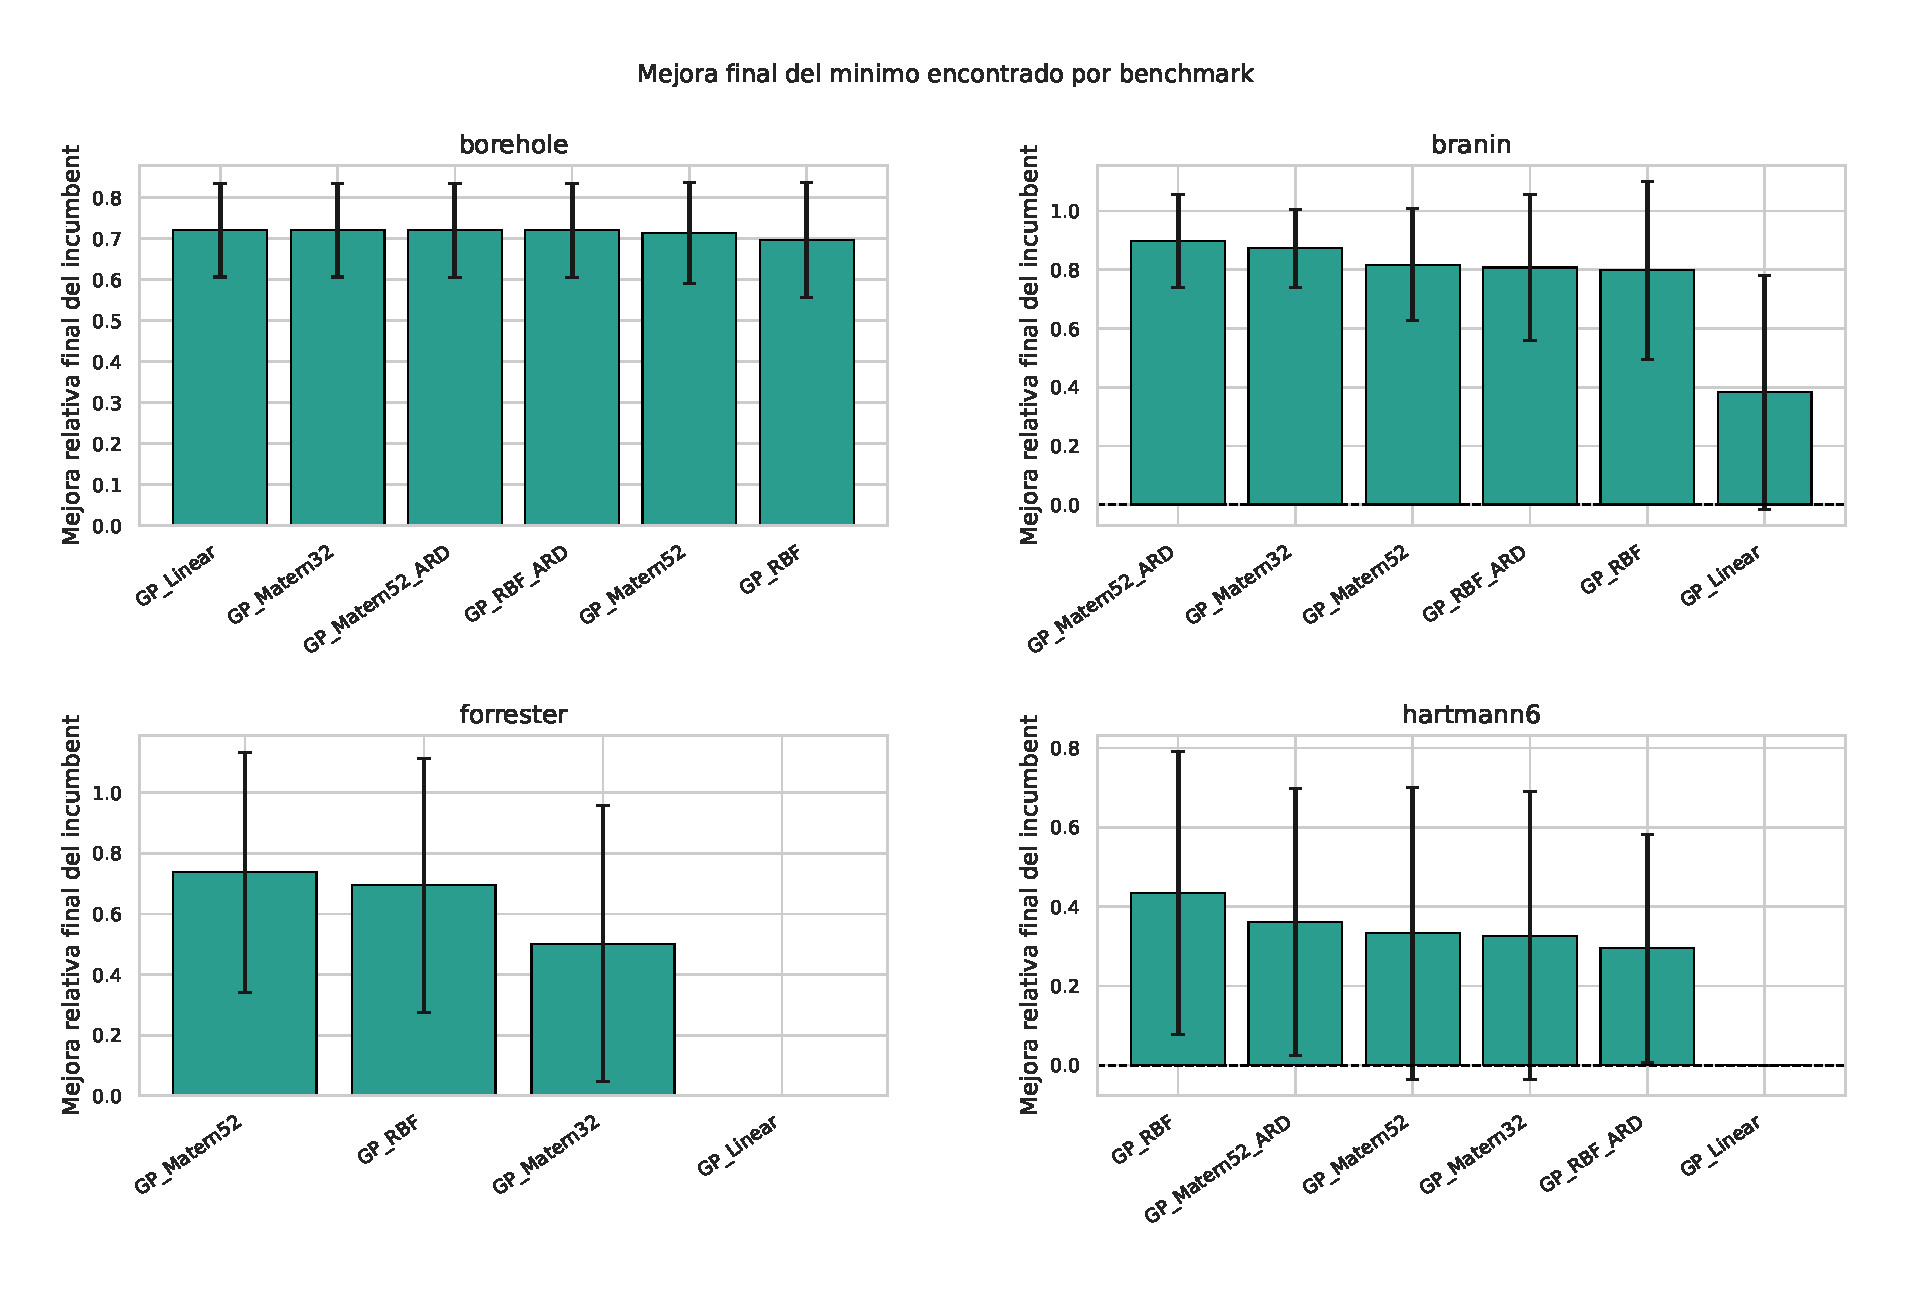
\includegraphics[width=0.9\textwidth]{assets/final_relative_incumbent_improvement_by_benchmark.eps}
\caption[Mejora final del mínimo encontrado]{Mejora relativa final del mínimo encontrado durante el proceso de \emph{infill}. En Forrester, Branin y Hartmann6 se representa la reducción relativa del \emph{gap} al óptimo. En Borehole, al no disponer de óptimo definido en la implementación, se muestra la reducción relativa del mejor valor limpio respecto al diseño inicial. Las barras indican la media y las líneas verticales la desviación típica sobre las trayectorias agregadas.}
\label{fig:app_final_relative_incumbent_improvement}
\end{figure}

La Figura~\ref{fig:app_final_relative_incumbent_improvement} resume el éxito de optimización del proceso de \emph{infill}, no la calidad predictiva global del modelo sustituto. En Branin se obtiene la mayor reducción media del \emph{gap} al óptimo, con GP\_Matern52\_ARD, seguida de Forrester con GP\_Matern52. Borehole también muestra una mejora fuerte, aunque en este caso se mide la reducción del mejor valor limpio porque no se dispone de un óptimo de referencia en la implementación. Hartmann6 presenta una mejora más moderada y con mayor variabilidad.

En conjunto, la figura confirma que EI permite encontrar mejores valores de la función objetivo en todos los benchmarks, pero también muestra que la magnitud de la mejora depende mucho del problema. Por ello, el \emph{incumbent} debe interpretarse como la métrica central del éxito de búsqueda, complementaria al MAE y al resto de métricas predictivas.


\section{Evolución relativa del MAE}
\label{app:evolucion_relativa_mae}

\begin{figure}[htbp]
\centering
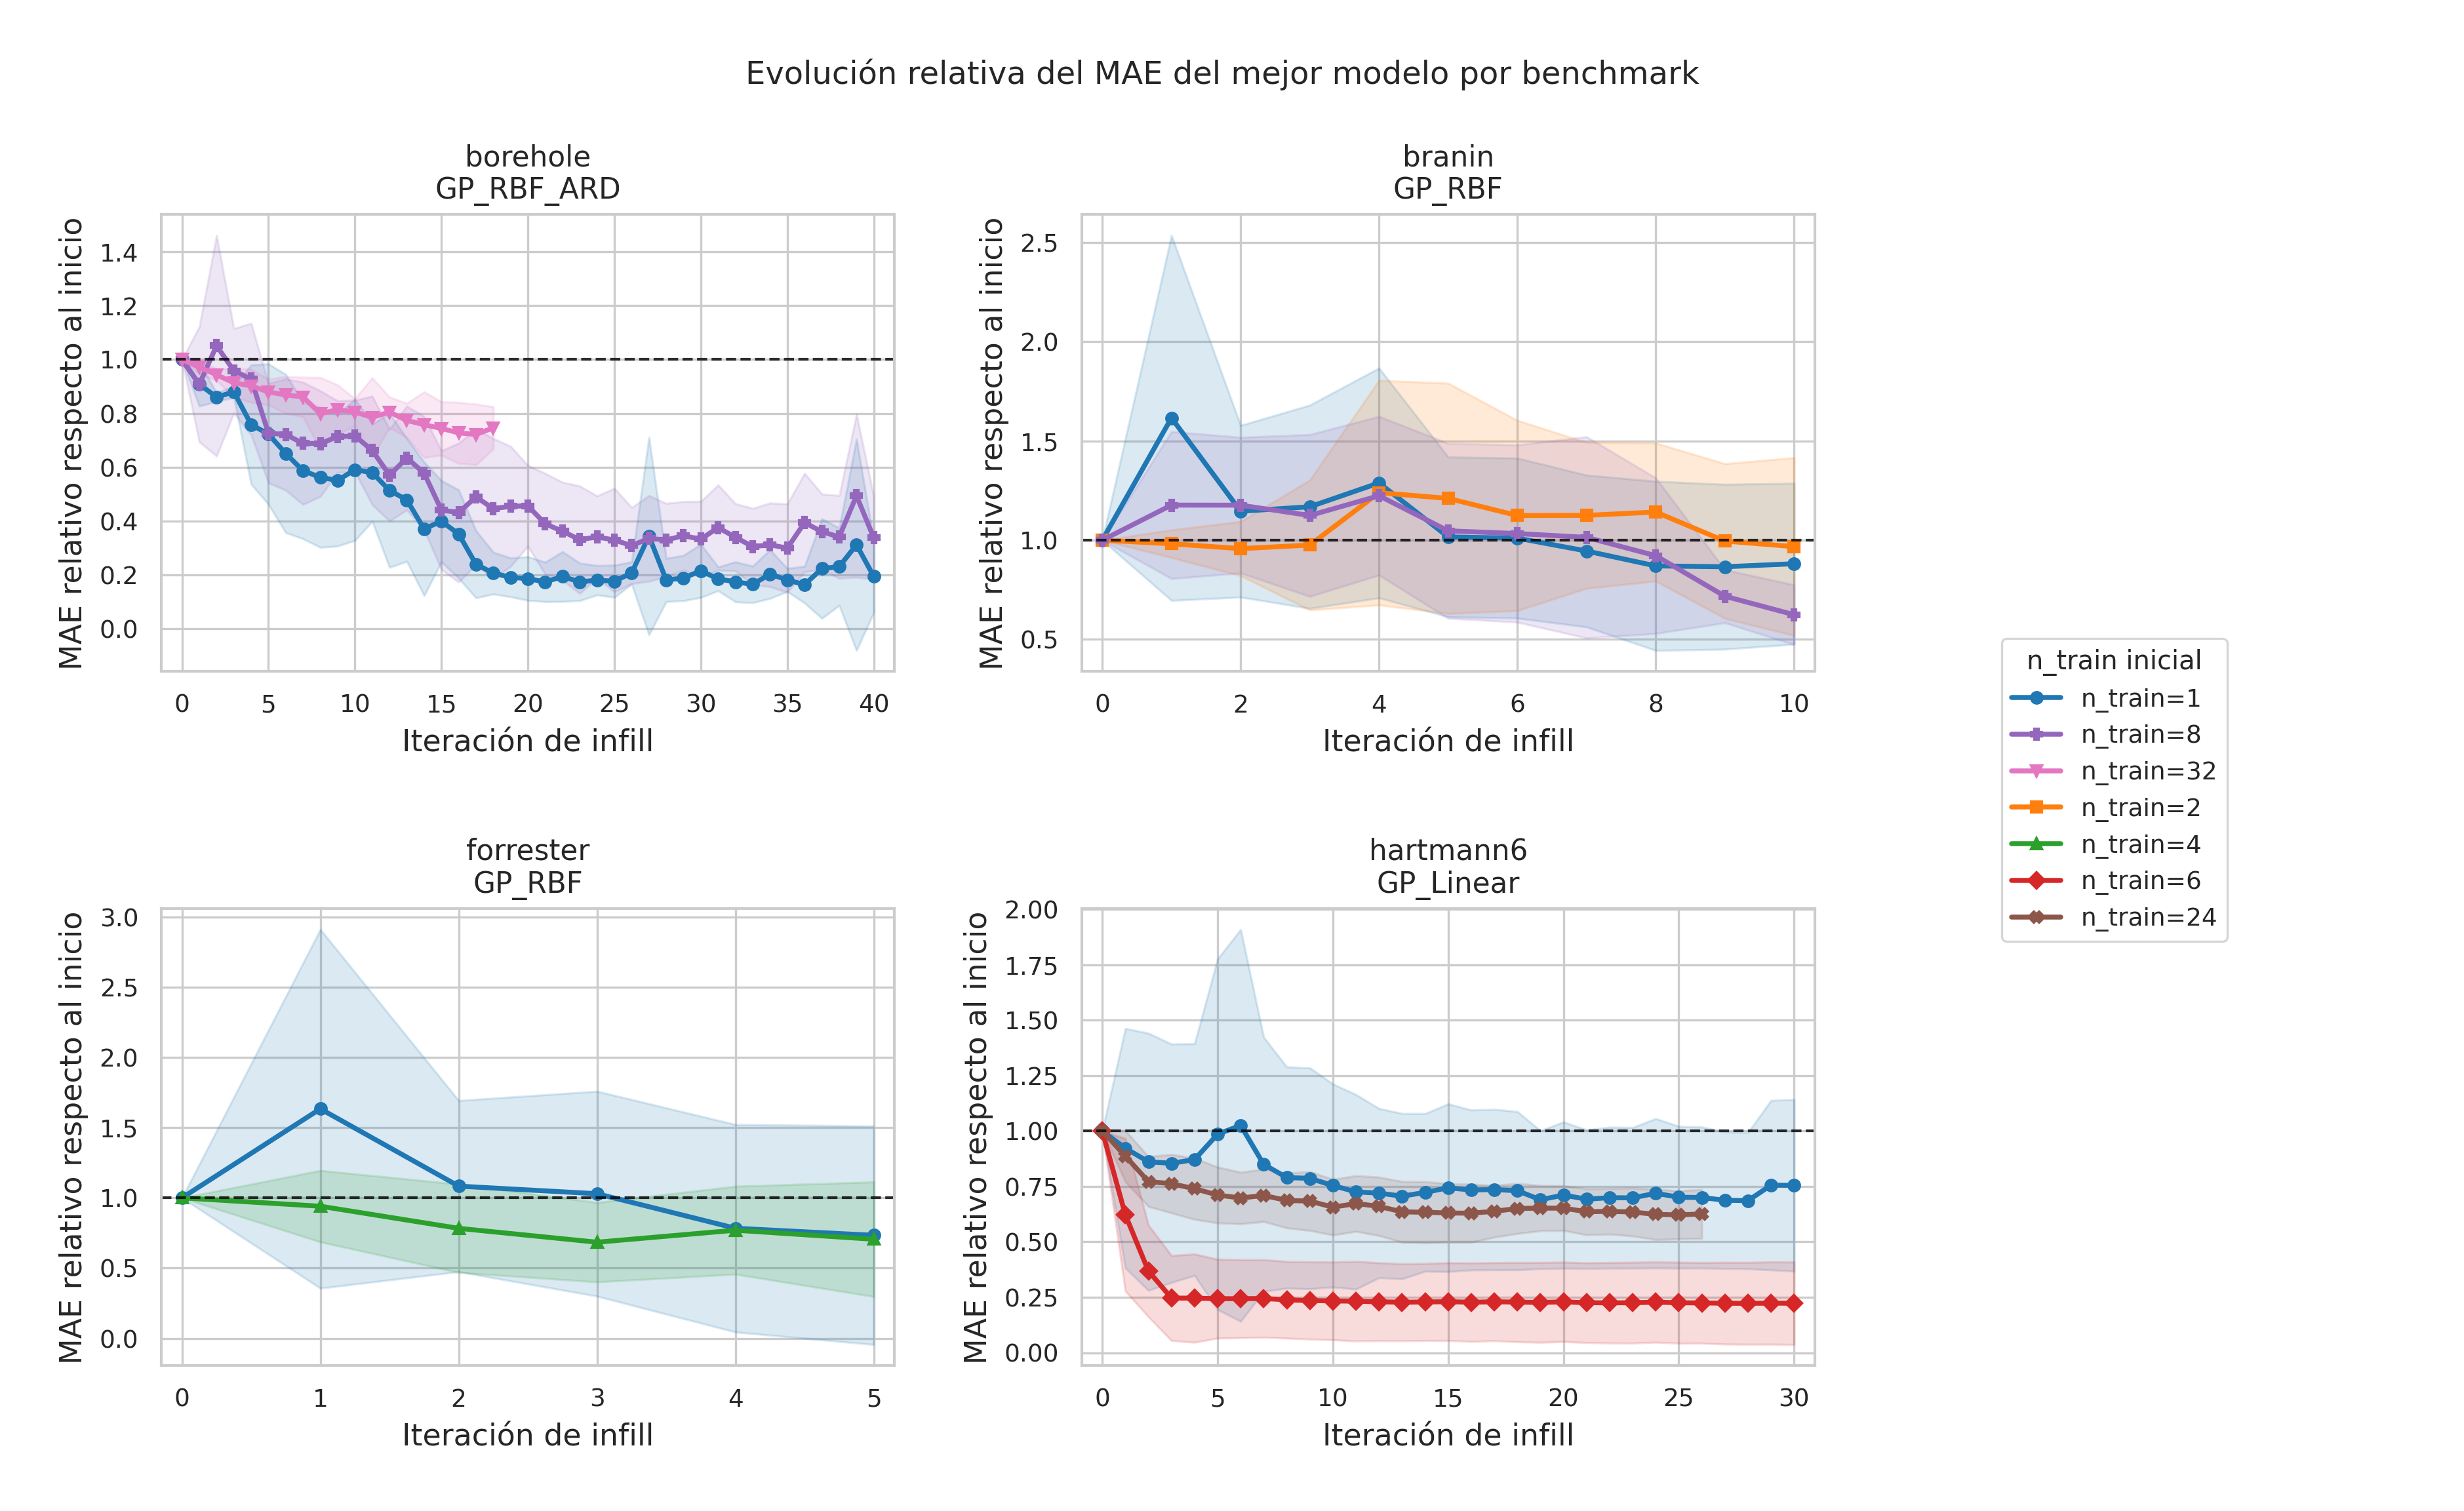
\includegraphics[width=\textwidth]{assets/evolution_relative_mae_best_model_by_benchmark.png}
\caption[Evolución relativa del MAE]{Evolución relativa del MAE para el mejor modelo predictivo de cada benchmark. La línea discontinua marca el valor inicial. Valores inferiores a 1 indican una reducción del error respecto al modelo entrenado únicamente con el diseño inicial.}
\label{fig:app_evolution_relative_mae_best_model}
\end{figure}

La Figura~\ref{fig:app_evolution_relative_mae_best_model} muestra la evolución del MAE relativo durante el proceso de \emph{infill} para el mejor modelo predictivo de cada benchmark. La línea discontinua en \(1\) representa el error del modelo entrenado solo con el diseño inicial; por tanto, valores inferiores a \(1\) indican una reducción del MAE y valores superiores reflejan un empeoramiento temporal.

El patrón más claro aparece en Borehole, donde GP\_RBF\_ARD reduce el error de forma sostenida, sobre todo cuando el diseño inicial es pequeño. En Hartmann6 también se observa una mejora rápida, especialmente para \(n_{\mathrm{train}}=6\), donde GP\_Linear alcanza una reducción marcada del MAE. En cambio, Branin y Forrester presentan trayectorias menos monótonas: algunas configuraciones empeoran al inicio antes de estabilizarse o mejorar. Esto indica que añadir puntos mediante EI no siempre reduce el error global de forma inmediata.

En conjunto, la figura muestra que el \emph{infill} puede mejorar la calidad predictiva del modelo sustituto, pero que esta mejora depende del benchmark, del tamaño inicial y del modelo. Además, el MAE relativo no debe confundirse con el éxito de optimización: EI selecciona puntos para mejorar la búsqueda del óptimo, no necesariamente para minimizar de forma monótona el error predictivo en todo el dominio.


\section{Diagnóstico predictivo y probabilístico}
\label{app:diagnostico_predictivo_probabilistico}
\begin{figure}[htbp]
\centering
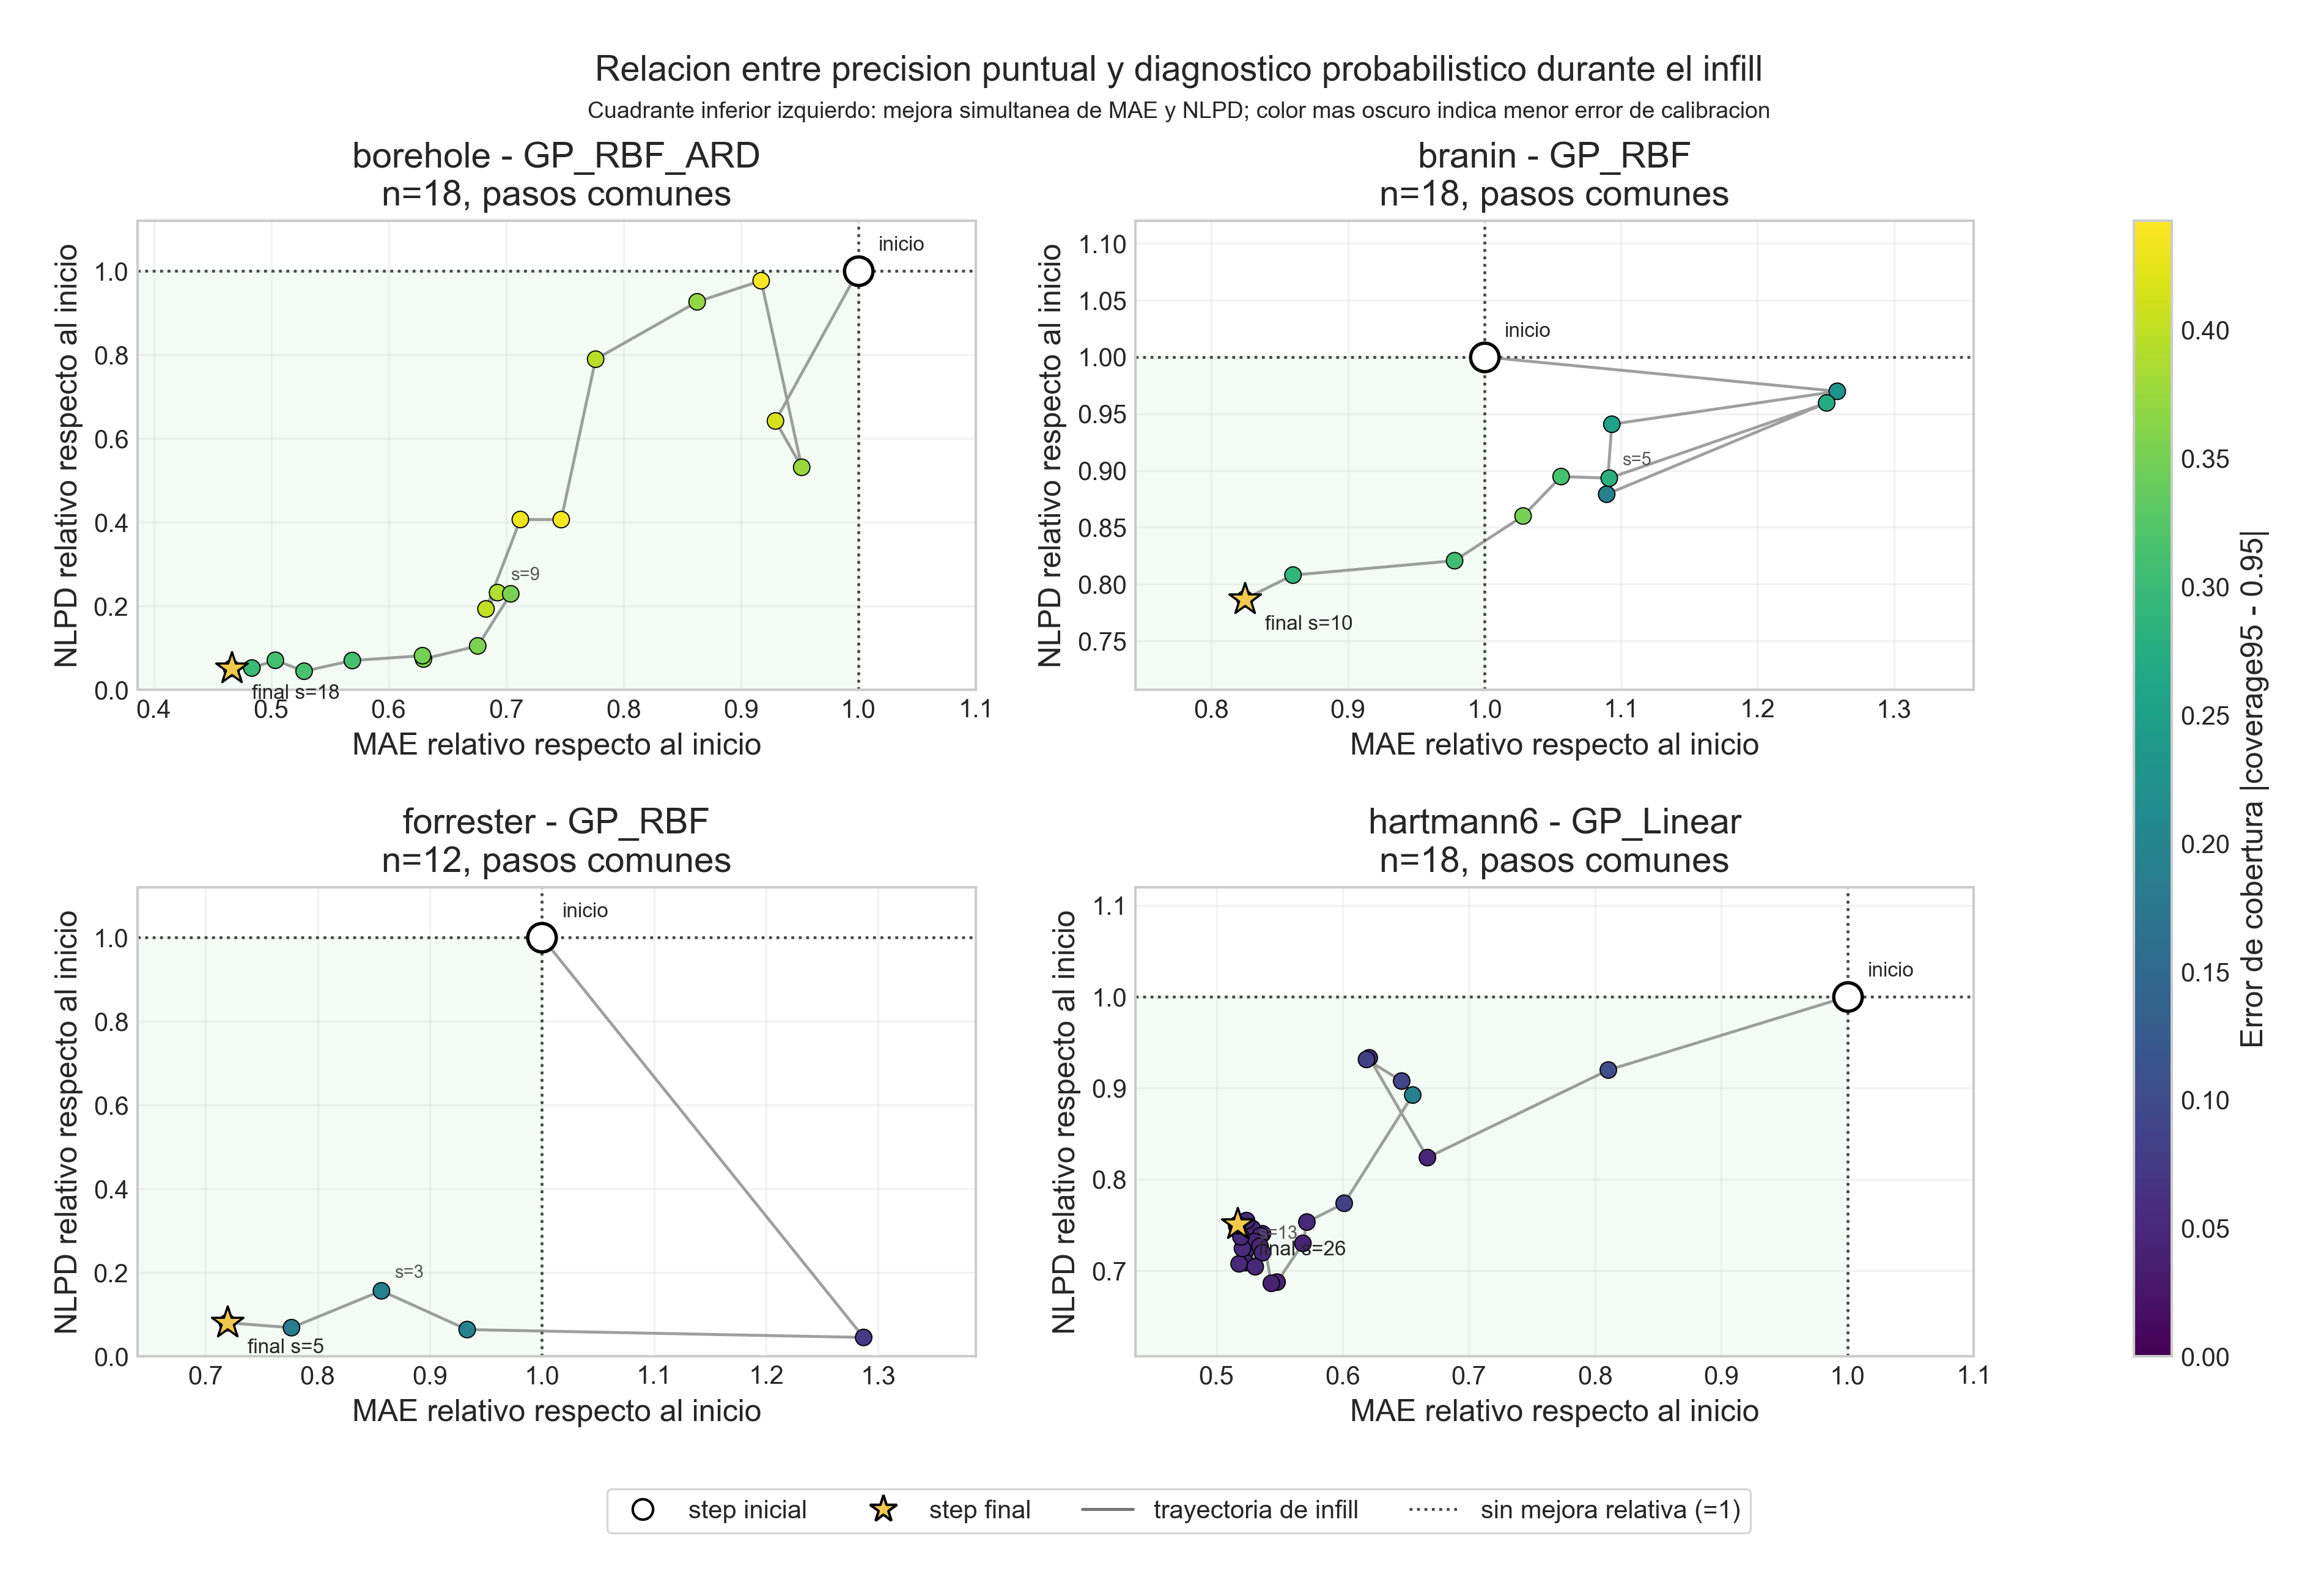
\includegraphics[width=\textwidth]{assets/mae_vs_probabilistic_diagnostics_by_step.png}
\caption[Diagnóstico predictivo y probabilístico]{Relación entre precisión puntual y diagnóstico probabilístico durante el proceso de \emph{infill}. El eje horizontal representa el MAE relativo respecto al inicio y el eje vertical el NLPD relativo. El cuadrante inferior izquierdo corresponde al caso deseable, con mejora simultánea en error puntual y diagnóstico probabilístico. El color indica el error de calibración de la cobertura al 95 \%, definido como \(\left|\mathrm{coverage}_{95}-0.95\right|\).}
\label{fig:app_mae_vs_probabilistic_diagnostics}
\end{figure}

La Figura~\ref{fig:app_mae_vs_probabilistic_diagnostics} relaciona la mejora en error puntual con la mejora del diagnóstico probabilístico durante el \emph{infill}. El eje horizontal muestra el MAE relativo y el eje vertical el NLPD relativo, ambos respecto al inicio. Por tanto, el cuadrante inferior izquierdo representa el caso deseable: menor error medio y mejor calidad probabilística que en el diseño inicial. El color añade una tercera lectura, el error de calibración de la cobertura al \(95\,\%\), donde tonos más oscuros indican intervalos mejor calibrados.

Los cuatro benchmarks terminan en la zona de mejora simultánea, aunque con matices. Borehole muestra la mejora más clara en MAE y NLPD, con un punto final cercano a \(0.47\) en MAE relativo y \(0.05\) en NLPD relativo; sin embargo, mantiene subcobertura, por lo que la incertidumbre no queda plenamente calibrada. Forrester también mejora de forma marcada en NLPD y de manera moderada en MAE. Branin presenta una mejora más suave y una trayectoria menos directa. Hartmann6 ofrece el comportamiento más equilibrado: reduce el MAE y mantiene una calibración cercana al \(95\,\%\).

La conclusión principal es que la mejora predictiva no debe evaluarse solo con MAE. Un modelo puede reducir el error medio y seguir proporcionando intervalos de incertidumbre mal calibrados. Por ello, esta figura complementa la evolución del MAE y justifica analizar conjuntamente precisión puntual, NLPD y cobertura predictiva.


\section{Efecto de las condiciones experimentales}
\label{app:efecto_condiciones_experimentales}
\begin{figure}[htbp]
\centering
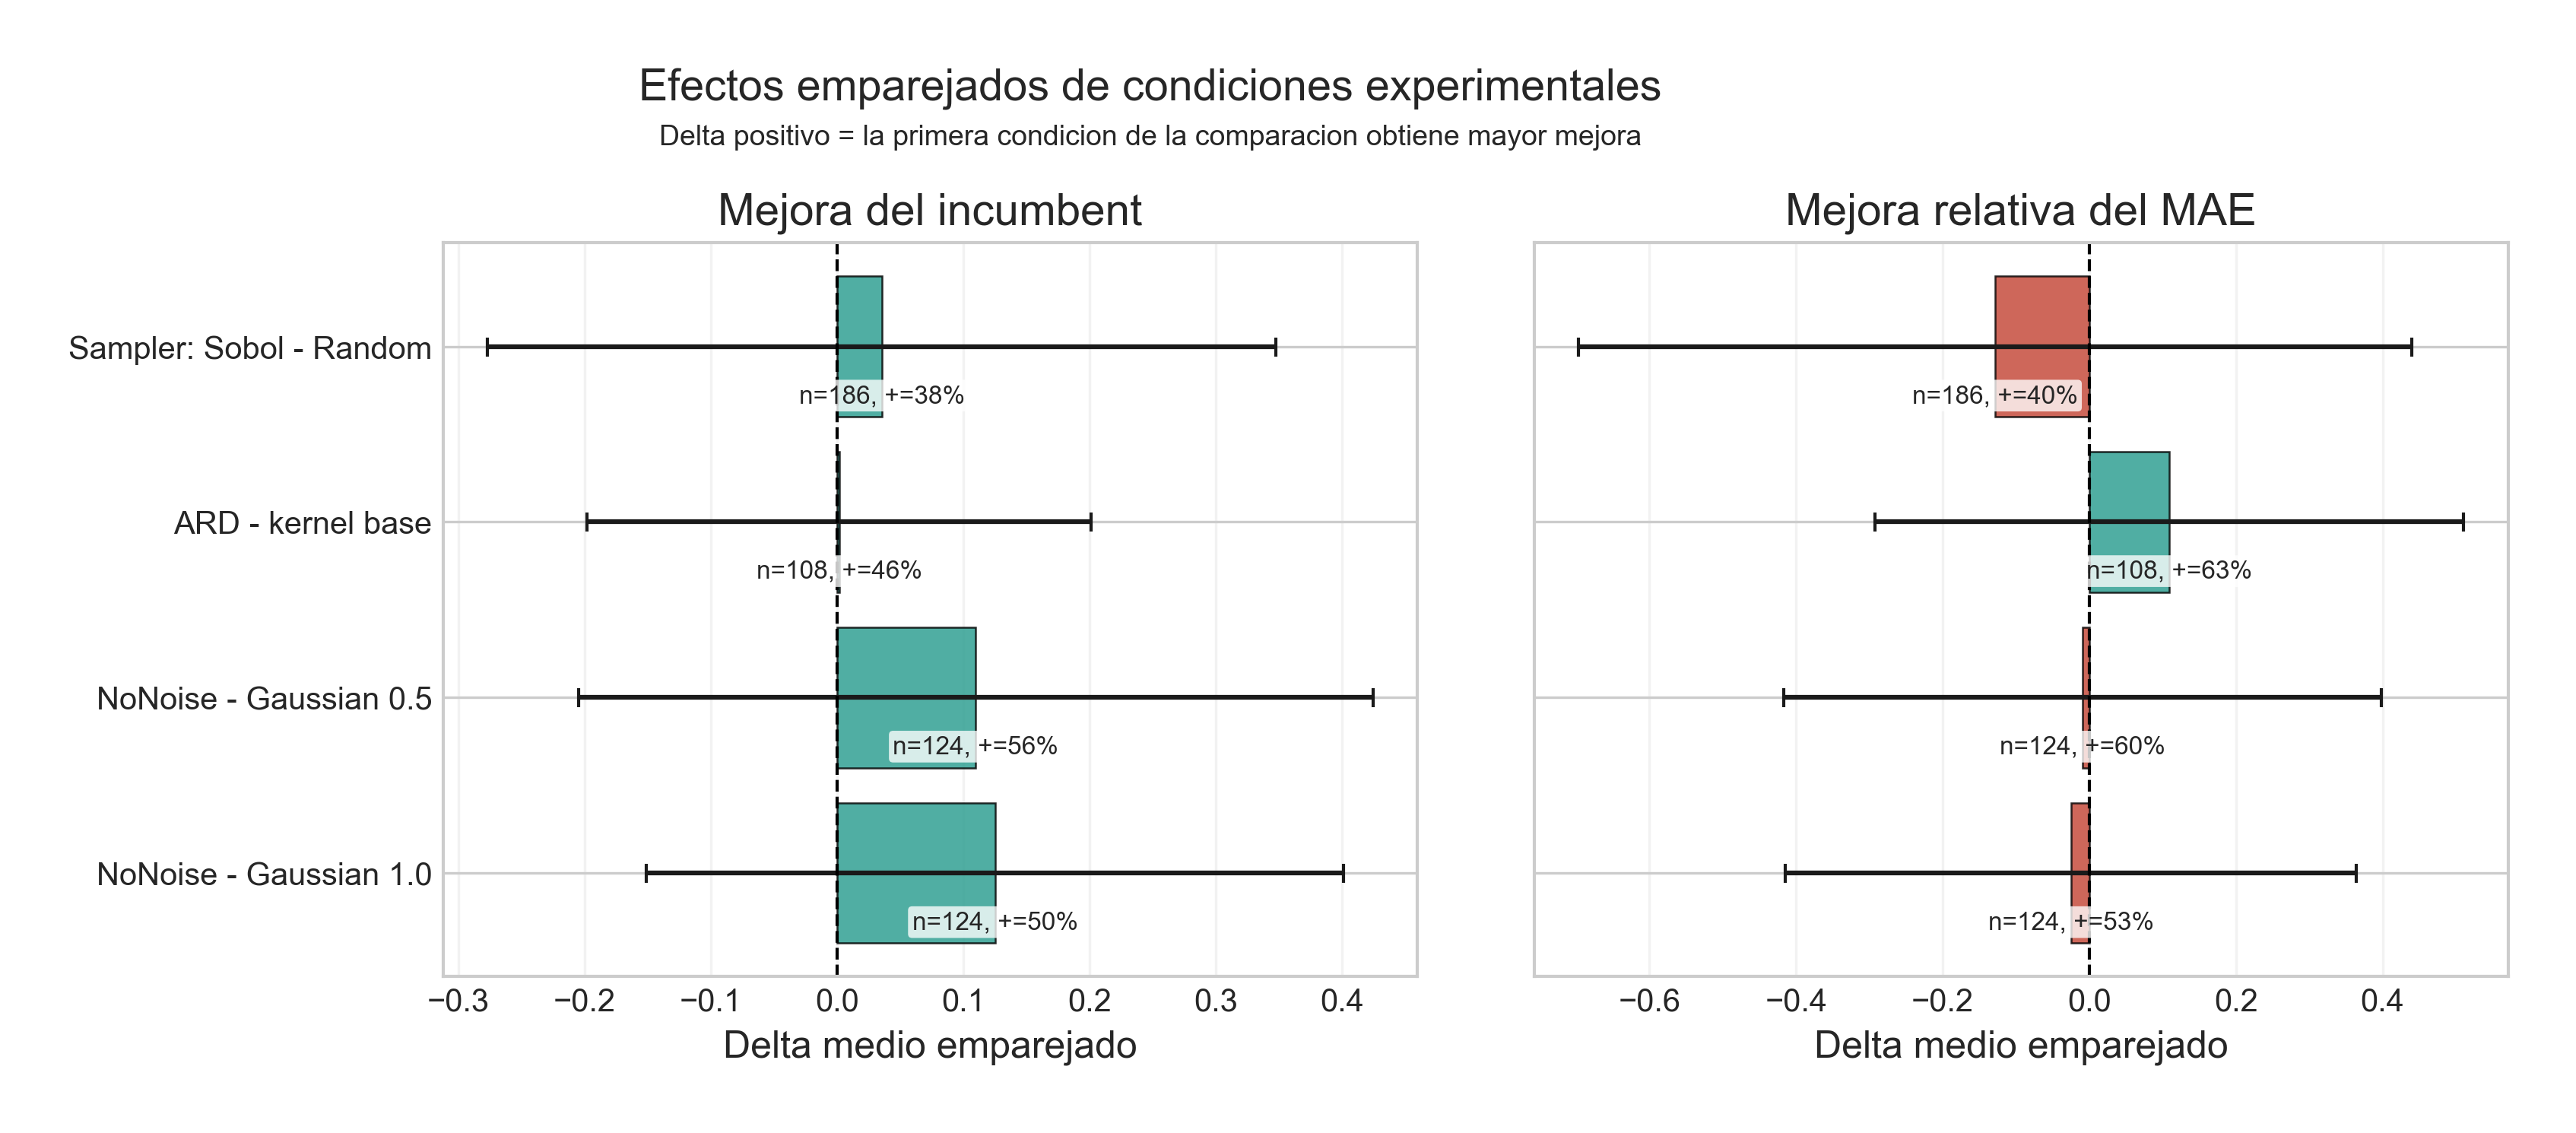
\includegraphics[width=\textwidth]{assets/factor_effects_paired_for_tfg.png}
\caption[Efecto de las condiciones experimentales]{Efectos emparejados de distintas condiciones experimentales sobre la mejora del mínimo encontrado y la mejora relativa del MAE. Un delta positivo indica que la primera condición de la comparación obtiene mayor mejora media. Las barras horizontales representan la desviación típica de los deltas emparejados.}
\label{fig:app_factor_effects_paired}
\end{figure}

La Figura~\ref{fig:app_factor_effects_paired} compara el efecto medio de distintas condiciones experimentales manteniendo emparejadas el resto de configuraciones. Los deltas son, en general, pequeños respecto a su variabilidad, lo que indica que ningún factor aislado domina de forma estable el resultado. En mejora del \emph{incumbent}, la ausencia de ruido muestra un efecto positivo moderado frente a ruido gaussiano, mientras que Sobol frente a aleatorio y ARD frente a kernel base presentan efectos débiles.

En MAE, ARD tiende a mejorar ligeramente el resultado medio, pero con alta dispersión. El muestreo Sobol no muestra una ventaja clara frente al aleatorio y el efecto del ruido sobre el MAE es pequeño. Por tanto, la figura sugiere que el comportamiento final depende más del benchmark y de la interacción entre condiciones que de una única decisión experimental aislada.
